\documentclass[11pt]{report}
 
 \usepackage[x11names,table]{xcolor}
 
\usepackage[spanish]{babel} %Español 
\usepackage{amsmath}
\usepackage{graphicx}
\usepackage{listings}
\usepackage{color}
\usepackage{vmargin}
\usepackage{hyperref}
\usepackage{graphbox}

\usepackage{chronology}
\usepackage{float}
\usepackage{pgfplots}
\usepackage{url}
\usepackage[utf8x]{inputenc}
\usepackage[TS1,T1]{fontenc}
\usepackage{array, booktabs}
\usepackage{caption}
\DeclareCaptionFont{blue}{\color{LightSteelBlue3}}

\newcommand{\foo}{\color{LightSteelBlue3}\makebox[0pt]{\textbullet}\hskip-0.5pt\vrule width 1pt\hspace{\labelsep}}
\newcommand{\lstfont}[1]{\color{#1}\scriptsize\ttfamily}

\graphicspath{ {Images/} }
 
%\setmargins{1.5cm}       % margen izquierdo
%{1.5cm}                  % margen superior
%{16cm}                 % anchura del texto
%{23.42cm}                % altura del texto
%{10pt}                   % altura de los encabezados
%{1cm}                    % espacio entre el texto y los encabezados
%{0pt}                    % altura del pie de página
%{2cm}                    % espacio entre el texto y el pie de página


\definecolor{dkgreen}{rgb}{0,0.6,0}
\definecolor{gray}{rgb}{0.5,0.5,0.5}
\definecolor{mauve}{rgb}{0.58,0,0.82}
\definecolor{purple}{rgb}{0.58,0,0.58}

\lstset{frame=single,
	language=C++,
	aboveskip=3mm,
	belowskip=3mm,
	showstringspaces=false,
	columns=flexible,
	basicstyle={\small\ttfamily},
	numbers=none,
	numberstyle=\tiny\color{gray},
	keywordstyle=\color{blue},
	commentstyle=\color{dkgreen},
	stringstyle=\color{mauve},
	breaklines=true,
	breakatwhitespace=true,
	tabsize=4,
	emph={
        cudaMalloc, cudaFree,
        __global__, __shared__, __device__, __host__,
        __syncthreads,
    },
	emphstyle=\color{purple},
	moredelim=[s][\ttfamily]{<<<}{>>>}
}
 
 
\def\code#1{\texttt{#1}}
	 
\setcounter{tocdepth}{5} %shows all levels incl. paragraph
\begin{document}
 


\begin{center}
    \rule[0.5ex]{\linewidth}{2pt}\vspace*{-\baselineskip}\vspace*{3.2pt}\\
    \rule[0.5ex]{\linewidth}{2pt}\\
    [2mm]
    {\textbf{\LARGE{Evaluación y aceleración del algoritmo Path tracing en arquitecturas heterogéneas}} }\\[3mm]
	\vspace{6.5mm}
    {\textbf{\large{Evaluation and acceleration of Path Tracing algorithm in heterogeneous architectures}} }\\[3mm]
    \rule[0.5ex]{\linewidth}{1pt}\vspace*{-\baselineskip}\vspace{3.2pt}
    \rule[0.5ex]{\linewidth}{2pt}\\
    \vspace{6.5mm}
    {\large Enrique de la Calle Montilla}
    \vspace{6.5mm}
    {\large\textsc{}}\\ %Nombres de los autores
    \vspace{5mm}
    
\includegraphics[width=0.5\textwidth]{logo}\\ %Logo de la UCM
    \vspace{6mm}
    {\large Trabajo de Fin de Grado en Ingeniería Informática\\   
    \textsc{Facultad de Informática}}\\
	\large Universidad Complutense de Madrid\\   
    \vspace{11mm}
    \begin{minipage}{10cm}
    \begin{center}
	Dirigido por\\
    Carlos García Sánchez\\
      \textbf{}\\
      \vspace{2mm}
    \end{center}
    \vspace{4mm}
    
    \end{minipage}\\
    \vspace{4mm}
    {\large\textsc{Madrid, 2020-2021}} %Fecha de finalización o presentación
    \vspace{12mm}
\end{center}

 
\tableofcontents

%\section{Dummy section}
%\subsection{Dummy subsection}
%\subsubsection{Dummy subsubsection}
%\paragraph{Dummy paragraph}

\chapter*{Resumen}
\markboth{RESUMEN}{RESUMEN}

En este trabajo se explica la implementación de Eleven Renderer, un motor de renderizado gráfico programado en C++ y CUDA de código abierto. Cuenta con todas las características necesarias para visualizar una escena 3d con relativa eficiencia y que hace uso de la arquitectura paralela que ofrecen los aceleradores gráficos. Además se acompaña con una evaluación y justificación de los detalles de la implementación además de ofrecer recursos en caso de querer ampliar información. Así pues, se espera que este trabajo sirva como breve guía y motivación para futuros programadores gráficos.

Eleven Renderer permite importar escenas desde la gran mayoría de software de edición 3d, aunque requiere de un proceso manual para adaptar el formato de la escena. Cuenta con una versión en oneAPI que puede ejecutarse en distintas plataformas sin requerir el uso de tarjetas gráficas de NVIDIA.


\chapter*{Abstract}
\markboth{ABSTRACT}{ABSTRACT}


\chapter*{Agradecimientos}
\markboth{AGRADECIMIENTOS}{AGRADECIMIENTOS}


\newpage

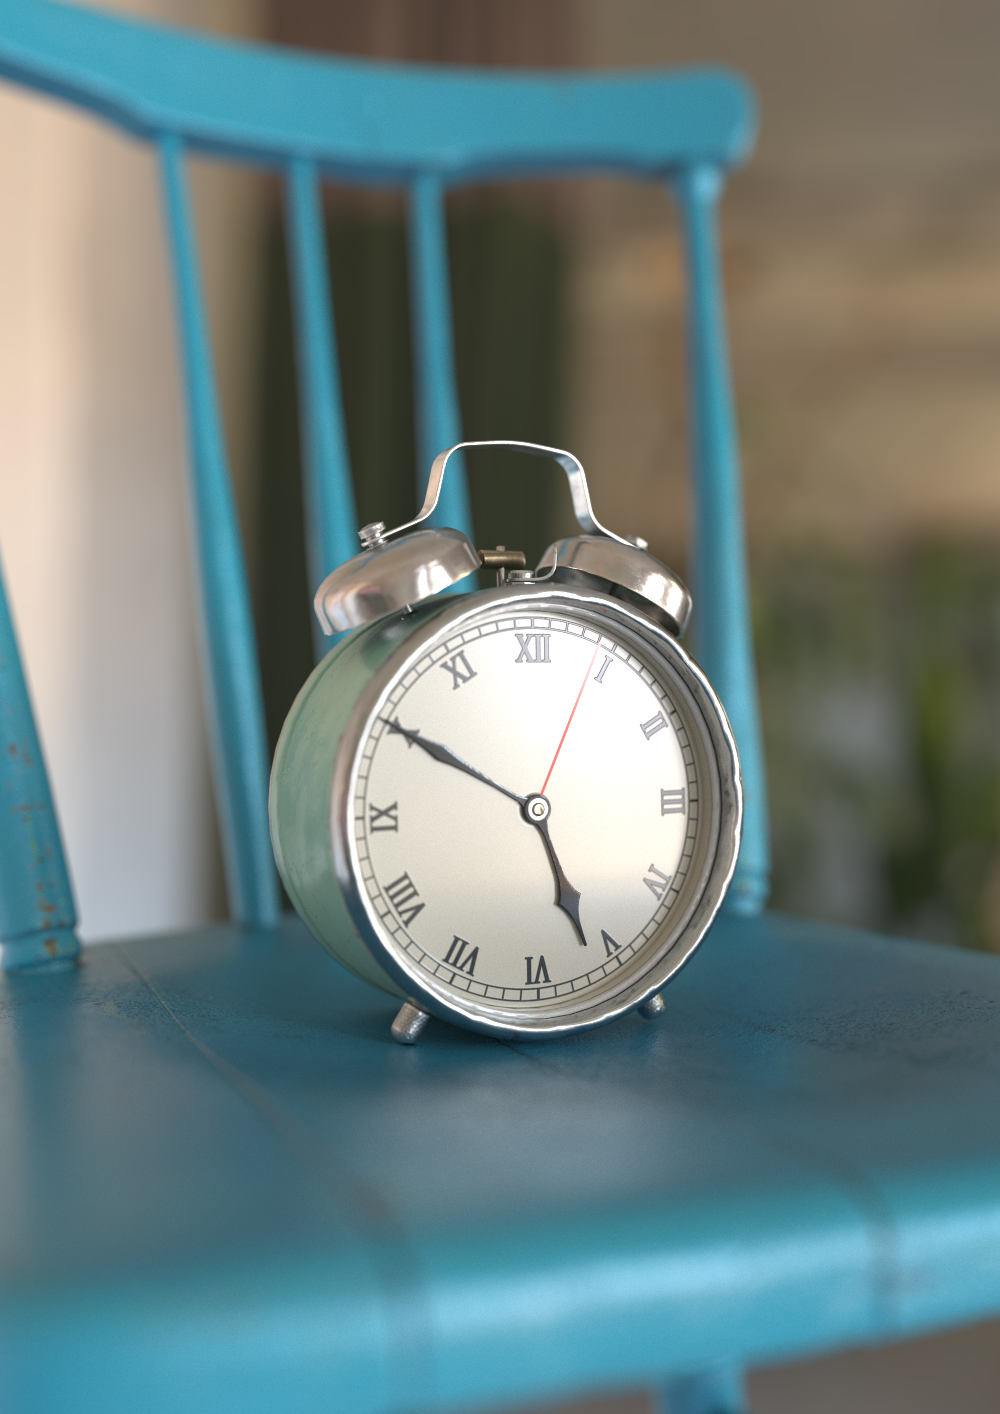
\includegraphics[
    width=1.45\textwidth,
    height=2\textwidth,
    align=t,
    smash=br,
    vshift=4cm,    
    hshift=-4.1cm
]{portada}

\scalebox{5}{\color{white}{Eleven Renderer}}


\chapter{Introducción}
	
El renderizado 3d es una técnica por la cual se representan los datos de geometrías tridimensionales en una pantalla en dos dimensiones. Existen distintas técnicas de renderizado tridimensional, siendo el trazado de rayos la más utilizada en la industria cinematográfica gracias a su excepcional fotorrealismo del cual carecen otras técnicas. Tan codiciada es esta técnica, que actualmente industrias realionadas con la visualización 3d como por ejemplo la industria de los videojuegos trata de replicarla y adaptarla en sus proyectos más modernos, con el fin de obtener mejor fidelidad visual.
El creciente interés ante el trazado de rayos ha provocado que compañías dedicadas al hardware gráfico dediquen parte de su desarrollo a la implementación del trazado de rayos en sus últimos modelos. Véase por ejemplo las últimas dos series de tarjetas gráficas de NVIDIA, siendo RTX (el nombre de las dos últimas series) acrónimo de "Ray Tracing Texel eXtreme". 

No obstante la implementación de este sistema de renderizado peca de una gran demanda computacional, es por ello que gran parte de los motores de renderizado orientados a la industria cinematográfica han sido adaptados para poder funcionar en aceleradores gráficos. Con la creciente capacidad computacional y las características fotorrealistas mencionadas anteriormente, los motores de renderizado de trazado de rayos han adquirido una especial importancia en el ámbito de la computación gráfica.



\section{Objetivos}

Este trabajo cubre las bases teóricas además de explicar la implementación en CUDA de un motor de renderizado fotorrealista con características a la orden del día de otros motores comerciales. Así pues este trabajo también hace hincapié en el análisis de dicha implementación en GPUs modernas, poniendo a prueba distintos parámetros y optimizaciones.

La implementación cuenta con características cercanas al estado del arte: es capaz de renderizar escenas del orden de millones de triángulos en tiempos razonables; usa un modelo de sombreado realista desarrollado por Disney; permite el uso de mapas de textura y además funciona en GPU.

Un aspecto importante en cuanto a la implementación es que se hace uso del menor número de librerías posibles, con el fin de indagar a fondo en la arquitectura de un motor de renderizado de Path Tracing de manera íntegra. Así pues se desmitifica el trabajo que normalmente se delega a las librerías gráficas, y se expondrá de manera clara el funcionamiento de cada pieza de un motor de renderizado de Path Tracing en GPU.

\chapter{Implementación básica de Path Tracing}
	
En este capítulo se procede a dar un esquema básico de los fundamentos de este algoritmo. El objetivo será así describir un motor de renderizado previo a cualquier optimización, que cuenta con las funcionalidades básicas para producir una imagen de una escena tridimensional simple.


\section{Esquema Path Tracing}
\label{pathtracingexplanation}


	\subsection{Aproximación de la ecuación de renderizado}
\[
{\displaystyle L_{\text{o}}(\mathbf {x} ,\omega _{\text{o}})=L_{\text{e}}(\mathbf {x} ,\omega _{\text{o}})\ +\int _{\Omega }f_{\text{r}}(\mathbf {x} ,\omega _{\text{i}},\omega _{\text{o}})L_{\text{i}}(\mathbf {x} ,\omega _{\text{i}})(\omega _{\text{i}}\cdot \mathbf {n} )\operatorname {d} \omega _{\text{i}}}
\]

La Ecuación de Renderizado \cite{kajiya1986rendering} aparece por primera vez en 1986 junto al algoritmo de Path Tracing, siendo este algoritmo una propuesta para resolverla. Es el pilar de la visualización 3d fotorrealista, ya que simula de una manera suficientemente precisa la interacción de la luz en una escena tridimensional. En este trabajo se utiliza una interpretación más moderna que sustituye términos como el ''término geométrico'' y adapta dicha ecuación al estado del arte.

La interpretación de esta ecuación es la siguiente: Para un punto $\mathbf {x}$ del espacio y un ángulo $\omega _{\text{o}}$ desde el cual se observa a dicho punto, cuál es la cantidad de energía lumínica que el observador recibe $L_{\text{o}}$. La interpretación geométrica se muestra en la \autoref{fig:renderingequation}.

El primer término $L_{\text{e}}(\mathbf {x} ,\omega _{\text{o}})$ indica la luz que dicho punto $\mathbf {x}$ emite, así pues se podrán modelar materiales que emitan luz propia y no dependan de energía externa.

El segundo término calcula toda la luz entrante y reflejada a través del ángulo $\omega _{\text{o}}$ por dicho punto $\mathbf {x}$, es por ello que integra todos los ángulos del hemisferio superior. Este segundo término se compone de tres coeficientes:

El primer coeficiente $f_{\text{r}}(\mathbf {x} ,\omega _{\text{i}},\omega _{\text{o}})$ es la función BRDF, la cual es dependiente del material e indica cuánta energía se refleja en dicho punto para las direcciones de entrada $\omega _{\text{i}}$ y salida $\omega _{\text{o}}$.

El segundo coeficiente $L_{\text{i}}(\mathbf {x} ,\omega _{\text{i}})$ hace referencia a toda la energía lumínica entrante de todas las direcciones posibles.

El tercer coeficiente $(\omega _{\text{i}}\cdot \mathbf {n})$ es el producto de la ley del coseno de Lambert \cite{lambert1760jh}, un escalar que atenúa los ángulos menos pronunciados con la normal de la superficie.

\begin{figure}[H]
    \centering
	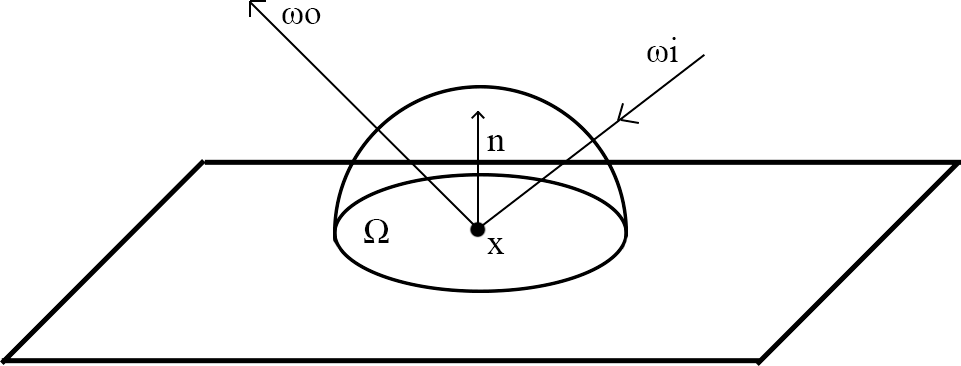
\includegraphics[width=0.5\textwidth]{renderingequation}
	\caption{Interpretación geométrica del término de integración de la ecuación de renderizado}
	\label{fig:renderingequation}
\end{figure}


	\subsection{Esquema de resolución}
	\label{subsec:montecarlo}
Kajiya \cite{kajiya1986rendering} propone junto a la ecuación el algoritmo de Path Tracing para resolverla. Este algoritmo se fundamenta en el método de Monte Carlo debido a la imposibilidad de resolver dicha ecuación de manera analítica.
Para aproximar una integral con el método de Monte Carlo, basta con muestrear aleatoriamente la función, y tras varias muestras es posible aproximar dicha integral. En la práctica, estas muestras son rayos con direcciones aleatorias y se tratará de aproximar la ecuación de renderizado. 

\[
{\int _{\Omega }f_{\text{r}}(\mathbf {x} ,\omega _{\text{i}},\omega _{\text{o}})L_{\text{i}}(\mathbf {x} ,\omega _{\text{i}})(\omega _{\text{i}}\cdot \mathbf {n} )\operatorname {d} \omega _{\text{i}} \approx \displaystyle \frac{1}{N}\sum\limits_{k=1}^{N}\frac{f_{\text{r}}(\mathbf {x} ,\omega _{\text{k}},\omega _{\text{o}})L_{\text{k}}(\mathbf {x} ,\omega _{\text{k}})(\omega _{\text{k}}\cdot \mathbf {n} )\operatorname {d} \omega _{\text{k}}}{p(\omega _{\text{k}})}}
\]

Así pues el procedimiento general es el siguiente:

\begin{enumerate}
	\item \hyperref[sec:calculatecameraray]{Calcular un rayo inicial desde la posición de la cámara a cada píxel del sensor de la cámara}.
	\item \hyperref[sec:throwray]{''Lanzar'' dicho rayo a la escena}.
	\item \hyperref[subsec:triintersection]{Comprobar la intersección de este rayo con el elemento más cercano al origen de este}. En caso de no intersecar se entiende que el rayo ha salido de la escena, de manera que se añade la luz del fondo a dicho camino y se salta al punto.
	\item Aplicar la reducción de energía pertinente a dicha intersección.
	\item Comprobar si se ha alcanzado el número máximo de rebotes, en caso negativo se calcula la dirección a la que rebota dicho rayo y se vuelve al paso 2.
	\item Se añade al píxel la luz que contiene dicho rayo.
\end{enumerate}

Este procedimiento queda más claro en la \autoref{fig:algorithmscheme} donde se utilizan los nombres de las funciones utilizadas en la implementación.

\begin{figure}[H]
    \centering
	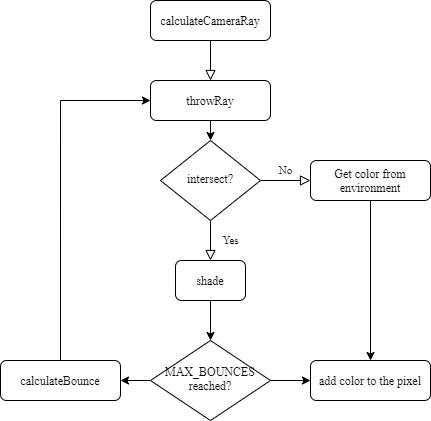
\includegraphics[width=0.5\textwidth]{algorithmscheme}
	\caption{Esquema Path Tracing}
	\label{fig:algorithmscheme}
\end{figure}



	\section{Pipeline}
		
En primer lugar es apropiado dar una visión de la estructura que se ha programado para Eleven Rendererer. Esta estructura está formada por una serie de clases y procedimientos cuyo objetivo es simular una escena 3D, transferirla a la GPU, ejecutar el algoritmo, transferir de vuelta el resultado como una imagen final y por último mostrar esta imagen al usuario. Además se ofrecerán distintas métricas con el fin de evaluar y conocer el estado del algoritmo para determinada escena.

\subsection{Preparado de escena}

El primer paso es preparar la escena a renderizar \code{Scene}. Una escena básica se compone de una cámara \code{Camera}, geometrías \code{MeshObject} y materiales \code{Material}.

La clase \code{Scene} contiene un array dinámico para cada conjunto de elementos, con sus pertinentes funciones de añadido. Por ejemplo, la función \code{addMeshObject()} lleva la cuenta de objetos en la escena y actualiza el ID de cada objeto a partir de esta cuenta. Además esta clase cuenta con una función denominada \code{Scene sceneBuilder(std::string path)} que cargará una escena localizada en un directorio. Más detalles sobre el formato de estas escenas se puede encontrar en \hyperref[sceneformat]{el manual ubicado en el anexo}

Los elementos básicos que almacena una escena son los siguientes:

\begin{itemize}

\item Cámaras \code{Camera}: consisten en una simulación aproximada de una cámara física real, así pues sus atributos serán: tamaño del sensor (en metros) \code{sensorWidth} y \code{sensorHeight}, distancia focal (en metros) \code{focalLength} y resolución (en píxeles) \code{xRes} e \code{yRes}. 

\item Geometrías \code{MeshObject}: son elementos que contienen un conjunto de triángulos \code{Tri} los cuales a su vez consisten en 3 puntos tridimensionales \code{Vector3 vertices[3]}.

\item Materiales \code{Material}: definen la manera en la que los fotones interactúan con ellos. En su forma más primitiva consisten en un color base, el cual absorberá ciertas longitudes de onda en mayor o menor medida. Para simplificar las computaciones, no es necesario calcular estas interacciones con todo el espectro electromagnético visible, basta con usar los tres colores primarios aditivos: rojo, verde y azul. Así, un color consiste en un vector \code{Vector3(R,G,B)}.

\end{itemize}

Una vez preparada la escena se inicia el proceso de renderizado. La función \code{startRender} prepara dos buffers en la CPU, \code{rawPixelBuffer} que recibirá los píxeles procedentes del algoritmo, previos a cualquier modificación y \code{beautyBuffer} que contendrá la imagen final preparada para ser mostrada en pantalla. 


El siguiente paso es transferir la escena a la GPU, donde se realizará el resto de computaciones más demandantes. Esto es realizado por la función \code{renderSetup}, que a través de las funciones de la API de CUDA \code{cudaMalloc} y \code{cudaMemcpy} copia la información de la escena y lleva la cuenta de la memoria transferida en las variables globales \code{textureMemory, geometryMemory}. La copia de memoria de la CPU a la GPU requiere de un tratado especial en cuanto a objetos con atributos refiere, requiriendo así una copia profunda de los atributos en formato array o punteros, además de un proceso posterior denominado ''pointer binding''. Este proceso como se aprecia en la \autoref{fig:pointerbinding} es necesario puesto que los objetos que hacen referencias a punteros al ser copiados a la GPU pierden dicha referencia al cambiar de contexto. 

Para ello si un objeto \code{Object} contiene un atributo \code{int* array}, habrá que asignar espacios de memoria diferentes para cada uno, copiar ambos independientemente y posteriormente, a través de la función \code{cudaMemcpy}, copiar la dirección del array a la dirección del atributo.

\code{cudaMemcpy(\&(Object->array), \&(array), sizeof(array*), cudaMemcpyHostToDevice);}

\begin{figure}[H]
    \centering
	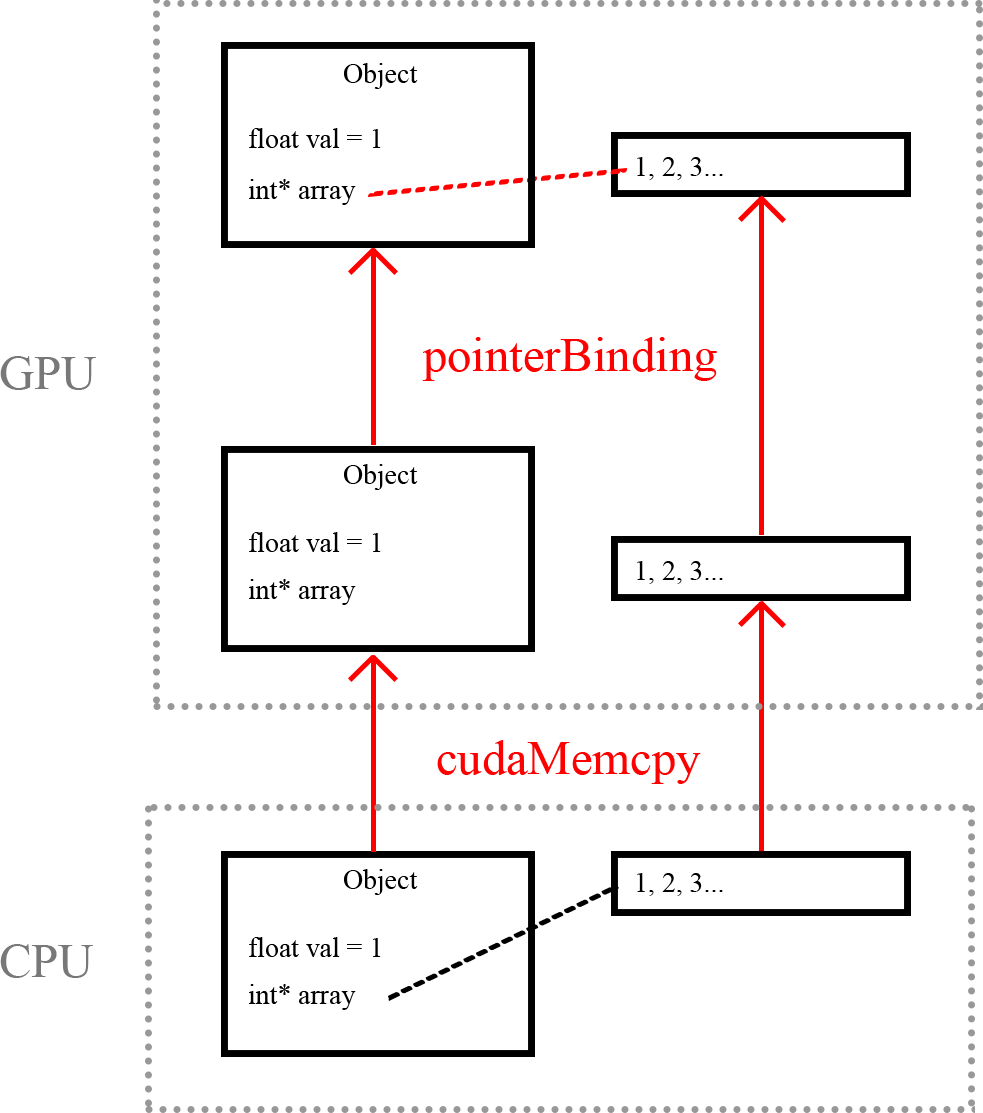
\includegraphics[width=0.5\textwidth]{pointerbinding}
	\caption{Pointer Binding}
	\label{fig:pointerbinding}
\end{figure}


La función \code{startRender}, tras realizar toda la copia de los elementos a la GPU, ejecuta un kernel que configura algunos parámetros iniciales. \code{setupKernel} cuyo código se muestra en \autoref{cod:setupkernel}, se ejecuta de manera síncrona y se hace cargo de inicializar los buffers de píxeles y contador de rayos, inicializar \code{curand} (la librería utilizada para generar números aleatorios en CUDA) y por último, enlazar cada \code{MeshObject} con sus pertinentes triángulos. Esto es llevado a cabo con un puntero a una posición de la lista global de triángulos, ya que por motivos que posteriormente se explican en \hyperref[BVH]{Estructuras de Aceleración} es conveniente almacenar todos los triángulos por separado. 


\begin{minipage}[c]{0.95\textwidth}
\begin{lstlisting}[label={cod:setupkernel}, caption={Kernel de configuración inicial}]
	
	__global__ void setupKernel() {

		int x = threadIdx.x + blockIdx.x * blockDim.x;
		int y = threadIdx.y + blockIdx.y * blockDim.y;

		int idx = (dev_scene_g->camera->xRes * y + x);

		if ((x >= dev_scene_g->camera->xRes) || (y >= dev_scene_g->camera->yRes)) return;

		dev_samples[idx] = 0;
		dev_pathcount[idx] = 0;

		cudaMemset(&dev_buffer[4 * idx], 0, sizeof(float) * 3); // RGB channels
		dev_buffer[4 * idx + 3] = 1; // Alpha channel

		curand_init(0, idx, 0, &d_rand_state_g[idx]);

		// Just one thread
		if (x == 0 && y == 0) {
			int triSum = 0;
			for (int i = 0; i < dev_scene_g->meshObjectCount; i++) {
				dev_scene_g->meshObjects[i].tris += triSum;
				triSum += dev_scene_g->meshObjects[i].triCount;
			}
		}
	}
\end{lstlisting}
\end{minipage}

Una vez la escena está correctamente configurada en la GPU, se crea un hilo nuevo que ejecutará en bucle el kernel de renderizado tantas iteraciones como muestras se hayan definido en los parámetros \code{RenderParameters}. Es necesario el uso de la librería \code{std::thread} para este proceso, ya que este bucle de llamadas a la GPU es un proceso bloqueante. El uso de dos hilos, uno para la ejecución de los kernels de renderizado y otro para la recolección de datos de la GPU de manera asíncrona, permite una previsualización dinámica del resultado del motor. Más detalles sobre este proceso se describen en el apartado \hyperref[progressiverender]{Renderizado Progresivo}.

En este punto, el algoritmo está ejecutándose en la GPU. Para mostrar el resultado se crea una ventana con la librería multiplataforma \code{SFML}. Esta librería permite mostrar en pantalla una imagen en formato RGB de 8 bits. Para poder adaptar el resultado del algoritmo a una imagen visible es necesario aplicar una serie de funciones de postprocesado. \code{getRenderData} se encarga de aplicar estas funciones y obtener una imagen postprocesada visible, también conocida en informática gráfica como "Beauty Pass".

Las funciones a ejecutar de postprocesado son las siguientes:

\begin{enumerate}
	
	\item \code{flipY}: Debido a la configuración de la cámara, los píxeles son calculados de abajo a arriba, es necesario entonces invertirlos en el eje Y.
	\item \code{clampPixels}: Es la forma más sencilla de mapeo de tonos, limitar los valores al rango [0-1].
	\item \code{applysRGB}: Los monitores no trabajan en un espacio de color lineal, por eso es necesario aplicar la curva de correción de gamma 2.2.
	\item \code{HDRtoLDR}: Por último, es necesario convertir el array de píxeles de punto flotante a bytes. Ya que los valores en punto flotante están en [0,1], basta con multiplicar por 255 y hacer un posterior truncamiento.

\end{enumerate}

Finalmente la librería de \code{SFML} se encarga de mostrar la imagen y superpone un texto con el número de muestras calculadas hasta el momento, obtenidas con \code{getSamples}.

\section{Acumulado de muestras}
	
Por cada píxel por el que se traza un camino es necesario añadir la radiación de dicho camino. Este píxel cuenta con radiación previa acumulada de las anteriores muestras.

\[{newAccumulatedLight = \frac{oldAccumulatedLight * samples}{samples + 1} + \frac{newLight}{samples + 1}}\]
	
Dicha radiación queda reflejada en cada píxel siguiendo el código mostrado en \autoref{cod:sampleaccumulation} donde \code{dev\_samples[]} es una variable global que almacena un contador con el número de muestras acumuladas hasta el momento para un píxel determinado y \code{dev\_buffer[]} almacena la radiación total por píxel hasta el momento. Por otro lado
la función \code{isnan} es necesaria para evitar errores numéricos, puesto que en determinadas escenas se han encontrado artefactos gráficos.

\begin{minipage}[c]{0.95\textwidth}
\begin{lstlisting}[label={cod:sampleaccumulation}, caption={Código para la acumulación de luz por cada píxel}]
	
	unsigned int sa = dev_samples[idx]; // sa is the number of samples accumulated for this pixel.
	
	if (!isnan(light.x) && !isnan(light.y) && !isnan(light.z)) {

        if (sa > 0) {
            dev_buffer[4 * idx + 0] *= ((float)sa) / ((float)(sa + 1));
            dev_buffer[4 * idx + 1] *= ((float)sa) / ((float)(sa + 1));
            dev_buffer[4 * idx + 2] *= ((float)sa) / ((float)(sa + 1));
        }

        dev_buffer[4 * idx + 0] += light.x / ((float)sa + 1);
        dev_buffer[4 * idx + 1] += light.y / ((float)sa + 1);
        dev_buffer[4 * idx + 2] += light.z / ((float)sa + 1);

        dev_samples[idx]++;
    }
	
\end{lstlisting}
\end{minipage}
	
\subsection{Renderizado Progresivo}
\label{progressiverender}
		
Una ventaja de los motores de renderizado más modernos es el renderizado progresivo. En este proceso, las muestras se van acumulando poco a poco a lo largo de la imagen hasta que terminan por converger. Esto difiere de los motores de renderizado por CPU tradicionales, que acumulan las muestras en secciones locales y una vez que acumulan las suficientes, pasan a la siguiente sección. Este trabajo utiliza una implementación progresiva con el fin de estar más cerca del estado del arte.

Este tipo de implementación se beneficia de la copia de datos asíncrona de la GPU. Mientras el kernel se ejecuta, un flujo de datos secundario hace la copia del buffer de la GPU en la CPU, pudiendo así actualizar la visualización del resultado varias veces por segundo.

Este flujo de datos secundario se implementa con el tipo de datos \code{cudastream\_t} de la API de CUDA. Son necesarios dos flujos, uno denominado \code{kernelStream} y otro denominado \code{bufferStream}. Los kernels de inicialización y renderizado corren en el primer flujo, mientras que la función que obtiene el buffer es ejecutada en el segundo flujo. El código \autoref{cod:getbuffer} muestra la copia asíncrona de los buffers a través de la función \code{cudaMemcpyFromSymbolAsync}. También se hace copia del buffer de la suma de rayos emitidos por píxel \code{pathcountBuffer} con el fin de realizar métricas de eficiencia.


\begin{minipage}[c]{0.95\textwidth}
\begin{lstlisting}[label={cod:getbuffer}, caption={Código para obtener los buffers de la GPU}]
	
	cudaError_t getBuffer(float* pixelBuffer, int* pathcountBuffer, int size) {

		cudaStreamCreate(&bufferStream);

		cudaError_t cudaStatus = cudaMemcpyFromSymbolAsync(pixelBuffer, dev_buffer, size * sizeof(float) * 4, 0, cudaMemcpyDeviceToHost, bufferStream);
		if (cudaStatus != cudaSuccess) {
			fprintf(stderr, "returned error code %d after launching addKernel!\n", cudaStatus);
		}

		cudaStatus = cudaMemcpyFromSymbolAsync(pathcountBuffer, dev_pathcount, size * sizeof(unsigned int), 0, cudaMemcpyDeviceToHost, bufferStream);
		if (cudaStatus != cudaSuccess) {
			fprintf(stderr, "returned error code %d after launching addKernel!\n", cudaStatus);
		}

		return cudaStatus;
	}
	
\end{lstlisting}
\end{minipage}

%@todo analisis de movimiento de datos de memoria.

\section{Trazado de rayo desde la cámara}
\label{sec:calculatecameraray}

Para simular el trazado del rayo desde la cámara hasta la escena, se simula de manera simplificada como haría una cámara estenopeica. Para cada píxel del sensor, se calcula su posición en el espacio a partir del tamaño del sensor. Esto quiere decir que el píxel (0,0) se encuentra en la esquina inferior izquierda de la ubicación física del sensor y el píxel (\code{xRes, yRes}) se encuentra en la esquina superior derecha. Puesto que no se está teniendo en cuenta la rotación de la cámara, la coordenada z del sensor se puede simplificar con la distancia de la cámara hasta el sensor.

Si se observa un sensor físico real, se puede ver como los píxeles del sensor tienen un área. En la anterior explicación se determina la posición de cada píxel, pero es necesario muestrear a lo largo de todo el área del píxel para simular la realidad, no solo el centro de cada uno. Es por ello que se añade un término aleatorio \code{rx, ry} que se encargará de distribuir las posiciones a lo largo de la zona de cada píxel.

\begin{minipage}[c]{0.95\textwidth}
\begin{lstlisting}[label={cod:cameraray}, caption={Trazado de rayo a cámara}]
	
	__device__ void calculateCameraRay(int x, int y, Camera& camera, Ray& ray, float r1, float r2) {

		// Relative coordinates for the point where the first ray will be launched
		float dx = camera.position.x + ((float)x) / ((float)camera.xRes) * camera.sensorWidth;
		float dy = camera.position.y + ((float)y) / ((float)camera.yRes) * camera.sensorHeight;

		// Absolute coordinates for the point where the first ray will be launched
		float odx = (-camera.sensorWidth / 2.0) + dx;
		float ody = (-camera.sensorHeight / 2.0) + dy;

		// Random part of the sampling offset so we get antialiasing
		float rx = (1.0 / (float)camera.xRes) * (r1 - 0.5) * camera.sensorWidth;
		float ry = (1.0 / (float)camera.yRes) * (r2 - 0.5) * camera.sensorHeight;

		// Sensor point, the point where intersects the ray with the sensor
		float SPx = odx + rx;
		float SPy = ody + ry;
		float SPz = camera.position.z + camera.focalLength;

		// The initial ray is created from the camera position to the sensor point. No rotation is taken into account.
		ray = Ray(camera.position, Vector3(SPx, SPy, SPz) - camera.position);
	}

\end{lstlisting}
\end{minipage}
	
\section{Intersección en la escena}
\label{sec:throwray}

Una vez se conoce el rayo primario que se lanza desde la cámara, es necesario determinar con qué objeto colisiona y la información de esa intersección. Esto se realiza por la función \code{throwRay} que, de forma ingenua, probará si el rayo intersecciona con cada triángulo de la escena y devolverá la intersección más cercana al origen de éste. En la \autoref{BVH} se explica un método para evitar tener que probar a intersecar cada triángulo.

\subsection{Intersección triángulo - rayo}
\label{subsec:triintersection}
	
El cálculo de la intersección de un rayo con un triángulo es una de las operaciones más fundamentales de este algoritmo. Esta operación toma como parámetros un triángulo \code{Tri} y un rayo \code{Ray} y ofrece como resultado si dicho triángulo y rayo intersecan en el espacio y además un objeto \code{Hit} el cual cuenta con información adicional de la intersección.

La información adicional que devuelve esta operación es la siguiente:

\begin{itemize}
	
	\item \code{int hit.objectID}: ID del objeto al que pertenece dicho triángulo.
	
	\item \code{Vector3 hit.position}: Posición en el espacio del punto de intersección entre el rayo y el triángulo.
	
	\item \code{Vector3 hit.normal}: Normal de la superficie, calculada a partir del producto vectorial de dos aristas del triángulo.
	
	\item \code{bool hit.valid}: Validez de una intersección, por defecto falso. Verdadero en caso de haber intersecado correctamente.

\end{itemize}

Para la implementación se ha hecho uso del algoritmo Fast Minimum Storage Ray/Triangle Intersection\cite{moller1997fast}. En este paper se explica detalladamente el algoritmo de intersección, mientras este trabajo se limita a implementar dicho algoritmo a partir de una adaptación de la implementación en C que el autor ofrece.
	
\begin{minipage}[c]{0.95\textwidth}
\begin{lstlisting}[label={cod:triintersection}, caption={Adaptación de código Fast Minimum Storage Ray/Triangle Intersection\cite{moller1997fast} a Eleven Renderer}]
	
	__host__ __device__ inline bool hit(Ray& ray, Hit& hit) {

		float EPSILON = 0.0000001;

        Vector3 edge1 = vertices[1] - vertices[0];
        Vector3 edge2 = vertices[2] - vertices[0];

        Vector3 pvec = Vector3::cross(ray.direction, edge2);

        float u, v, t, inv_det;

        float det = Vector3::dot(edge1, pvec);

        inv_det = 1.0 / det;

        if (det > -EPSILON && det < EPSILON) return false;

        Vector3 tvec = ray.origin - vertices[0];

        u = Vector3::dot(tvec, pvec) * inv_det;
        if (u < 0.0 || u > 1.0)
            return false;

        Vector3 qvec = Vector3::cross(tvec, edge1);
        v = Vector3::dot(ray.direction, qvec) * inv_det;
        if (v < 0.0 || (u + v) > 1.0)
            return false;

        t = Vector3::dot(edge2, qvec) * inv_det;

        if (t < 0) return false;

        Vector3 geomPosition = ray.origin + ray.direction * t;
		Vector3 geomNormal = Vector3::cross(edge1, edge2).normalized();
		
		hit.normal = geomNormal;
		hit.position = geomPosition;
		hit.valid = true;
		hit.objectID = objectID;

        return true;
	}

\end{lstlisting}
\end{minipage}

\subsection{Kernel principal}
	
El kernel de renderizado \code{renderingKernel} se encarga de ejecutar el algoritmo descrito en la \autoref{fig:algorithmscheme}, donde el número máximo de rebotes es una constante definida en tiempo de compilación como \code{MAX\_BOUNCES}. La paralelización se hace a nivel de píxel, aunque existen distintos tipos de paralelización aplicable.

Este tipo de paralelización cuenta con la ventaja de ofrecer localidad espacial hasta el primer rebote. Para escenas abiertas, la gran mayoría de los bloques no sufrirán del fenómeno de ''branching'', ya que los píxeles más  . Este método cuenta con limitaciones tras realizar un rebote aleatorio, es común que los propios hilos divergen ya que puede que algunos hilos realicen un solo rebote mientras que otros realizen \code{MAX\_BOUNCES}. 

La ejecución de un kernel en CUDA debe estar acompañada de dos parámetros: el número de bloques y el número de hilos. En este caso, los bloques estánd distribuidos uniformemente a lo largo de la imagen como bloques bidimensionales de \code{THREADSIZE * THREADSIZE} píxeles. Estos parámetros se definen en \code{cod:kernelpars}.

\begin{minipage}[c]{0.95\textwidth}
\begin{lstlisting}[label={cod:kernelpars}, caption={Selección de parámetros para el kernel principal}]
	
    int tx = THREADSIZE;
    int ty = THREADSIZE;

    dim3 numBlocks(scene->camera.xRes / tx + 1, scene->camera.yRes / ty + 1);
    dim3 threadsPerBlock(tx, ty);
	
\end{lstlisting}
\end{minipage}

Resulta interesante conocer el número de hilos óptimo por cada bloque, por lo que se han evaluado distintos tamaños de bloque en la \autoref{fig:threadsize}. En esta figura aparece por primera vez el término kPath/s. Como la eficiencia es un campo esencial en el renderizado 3d, Eleven renderer cuenta con unas pocas funciones que dan una breve información del estado actual del motor. Uno de estos datos es el número global de caminos que se trazan por segundo. La medida kPath/s es útil de manera comparativa para una misma escena, ya que indica el rendimiento general del motor. En el caso de la comparativa del número de hilos, aquellas ejecuciones de 8 hilos por dimensión, son las que han mostrado mayor número de caminos trazados por segundo, de manera que este es el número óptimo y el usado para el resto de la implementación.

\begin{figure}[H]
\centering
\begin{tikzpicture}
\begin{axis}[
    axis y line = left,
    xlabel = \(THREADSIZE\),
    ylabel = {\(KPaths/s\)},
	ylabel style={yshift=0.5cm},
	scaled y ticks=false
]

\addplot[smooth, blue]
coordinates{(1,3517) (2, 7544) (4, 12851) (8, 15480) (16, 14114)};
\end{axis}
\end{tikzpicture}
\caption{Comparación eficiencia con tamaño de bloque}
\label{fig:threadsize}
\end{figure}



\chapter{Mejoras estructurales}
	
	\section{Desenfoque: Modelo de lente fina}
	
	Hasta ahora se ha estado utilizando un modelo de cámara ideal denominado cámara estenopeica. Esta cámara tiene la particularidad de tener un enfoque perfecto siempre, siendo una propiedad indeseada en un motor de renderizado fotorrealista, ya que la mayoría de las cámaras reales incluyen lentes en su estructura que desvían los rayos de luz gracias a la difracción del cristal, enfocando a determinada distancia, y desenfocando el resto de la escena. El hecho de poder enfocar a una distancia determinada permite hacer énfasis en un sujeto de la escena, y desenfocar el resto. Este efecto se conoce como ``Bokeh`` y es muy deseado en un motor de renderizado, puesto que es un recurso cinematográfico muy atractivo visualmente.

	Para solventar el problema del enfoque perfecto se va a hacer uso de un modelo de cámara denominado modelo de lente fina. Este modelo es una simplificación de lo que sería una simulación física de unas lentes reales. Al simplificar los cálculos, se pierden artefactos y desperfectos deseados como la aberración cromática o la distorsión de lentes, pero a cambio se obtiene la simplicidad de implementación.

	Para activar este efecto, es necesario compilar con la constante \code{BOKEH} definida. Esto desbloqueará la parte de código que hace el cálculo del desenfoque. 
	
	Este nuevo método añade a la clase \code{Camera} dos nuevas variables, por un lado \code{focusDistance} y por otro lado \code{aperture}. La primera define la distancia a la que se encuentra el plano de enfoque, y la segunda, la apertura en f-stops del iris de la cámara. 

	El procedimiento para calcular los rayos emitidos por el nuevo modelo de cámara es el siguiente:

	1: Se calcula el rayo original del método anterior, desde la cámara hasta el sensor.
	
	2: Se calcula la intersección de dicho rayo con el plano de enfoque, situado a la distancia \code{focusDistance}. La intersección se denomina \code{focusPoint}.
	
	3: En vez de emitir e rayo desde el punto de la cámara, se elige un punto aleatorio en el iris \code{iRP} y se emite un rayo desde ahí hasta el punto de enfoque \code{focusPoint}. Este nuevo rayo será un rayo bajo el modelo de cámara de lente fina. Los elementos situados a la distancia de enfoque \code{focusDistance} serán más nítidos que aquellos que no lo estén.

\begin{lstlisting}
	
	#if BOKEH
	
    float rIPx, rIPy;

    // The diameter of the camera iris
    float diameter = camera.focalLength / camera.aperture;

    // Total length from the camera to the focus plane
    float l = camera.focusDistance + camera.focalLength;

    // The point from the initial ray which is actually in focus
    Vector3 focusPoint = ray.origin + ray.direction * l;

    // Sampling for the iris of the camera
    uniformCircleSampling(r3, r4, r5, rIPx, rIPy);

    rIPx *= diameter * 0.5;
    rIPy *= diameter * 0.5;

    Vector3 orig = camera.position + Vector3(rIPx, rIPy, 0);

    //Blurred ray
    ray = Ray(orig , focusPoint - orig);

#endif 

\end{lstlisting}

	\begin{figure}
		\centering
		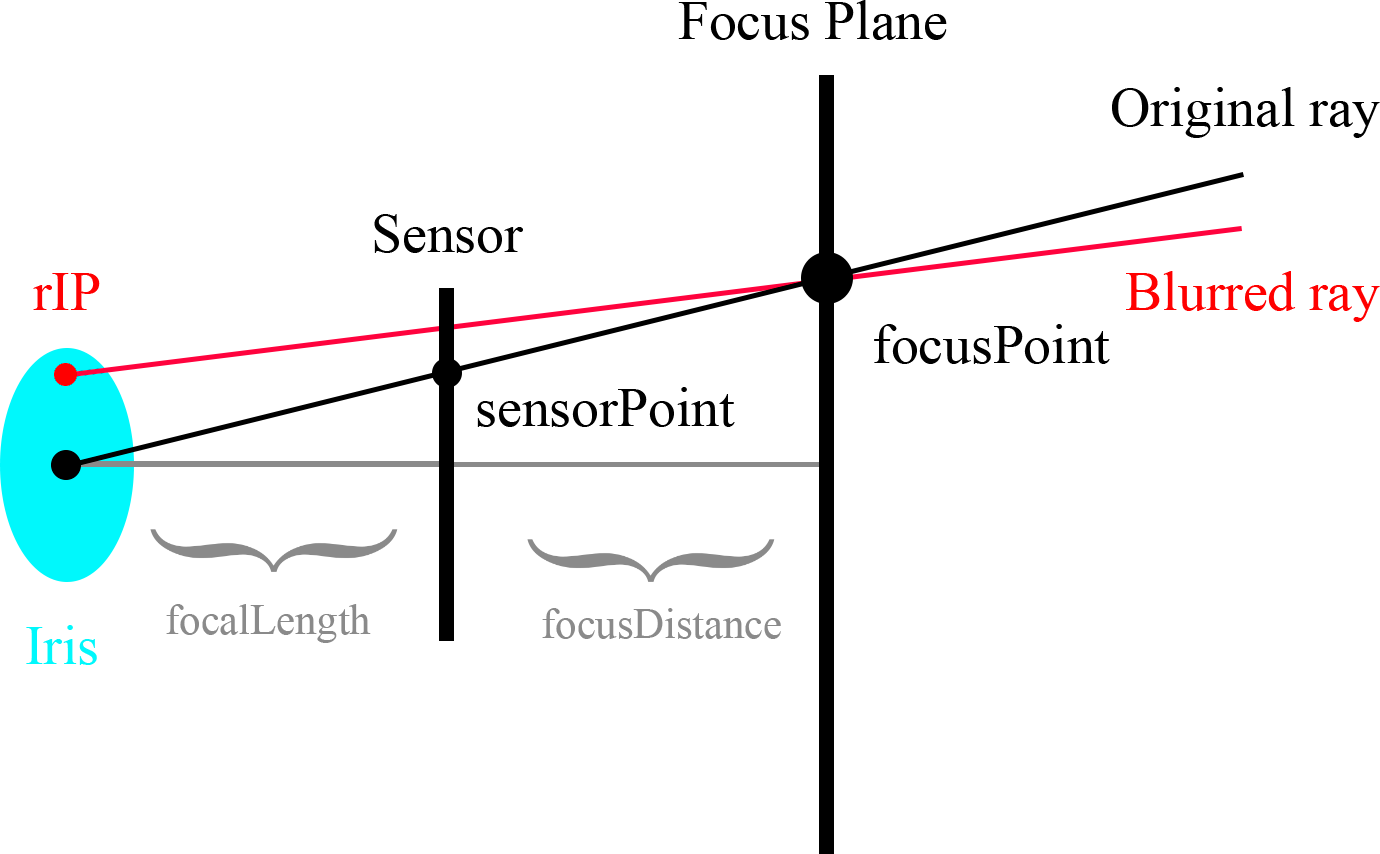
\includegraphics[width=0.7\textwidth]{blurring}
		\caption{}
		\label{fig:label}
	\end{figure}
	
	
	\section{Iluminación}
	
	En la implementación básica solo se hacía uso de luz ambiental para iluminar la escena. Se puede hacer uso de distintos mecanismos de iluminación para dar mayor riqueza visual. A continuación se detallan los tipos de luces implementadas.
	
	\begin{itemize}
		
	\item Luces de punto:

	Las luces de punto son quizá el elemento más simple de iluminación. Consisten en un punto sin volumen el cual emite radiación lumínica de manera uniforme. Esta radiación se desvanece de manera cuadrática. Debido a que son puntos infinitesimalmente pequeños, jamás serán alcanzados por los fotones emitidos desde la cámara, de manera que requieren un procesamiento especial explicado posteriormente en \autoref[sec:mi]{Muestreo por importancia}.

	Una luz de punto viene definida por tres atributos: Color, intensidad y posición. La energía lumínica viene dada por la ecuación:
	
	\item Materiales emisivos:

	Cuando un objeto es alcanzado por un rayo, lo más común es que se reste energía a dicho rayo debido a la absorción del material. Otra opción es sumarle energía. Si esto ocurre, se pasará a considerar a ese objeto como otra fuente de luz más.

	La energía sumada a dicho rayo será obtenida de una textura denominada emisión del material a través del mapeo correspondiente del punto de intersección, multiplicada así por un factor de intensidad.

	\item IBL (Image Based Lightning):

	La iluminación basada en imagen ha sido uno de los elementos más relevantes en las técnicas para el renderizado fotorrealista. Se utiliza ampliamente en la industria cinematográfica debido a la complejidad visual que aporta a una escena 3D y debido a que permite captar la iluminación de entornos reales y posteriormente añadirla en escenas digitales. El hecho de poder trasladar la iluminación a un escenario virtual, facilita la composición de modelos tridimensionales en películas y series de televisión donde es necesario juntar una grabación real con un elemento generado por ordenador.

	Esta técnica se basa principalmente en usar una fotografía de 360 grados como fuentes de luz formando una esfera alrededor de la escena. Estas fotografías son conocidas como HDRI (Imagen de Alto Rango Dinámico). A diferencia de las imágenes tradicionales las cuales normalmente tienen 8 bits de resolución por canal de color, las imágenes HDRI cuentan con valores de punto flotante. Esto es debido a que su uso no es meramente la visualización de estas en pantallas de 8 bits de resolución por color como la mayoría de imágenes, sino que el valor de cada píxel será utilizado para realizar las operaciones pertinentes para iluminar la escena.

	La implementación de esta técnica en el motor de render viene dada por el uso de una textura en formato .hdr (imágenes en punto flotante), o un color plano. En caso de utilizar una textura, se considerará cada píxel como una pequeña fuente de luz direccional en el infinito, orientada hacia el centro de la escena. 

	Los rayos que no interseccionan con nada se consideran que interseccionan en el infinito con el HDRI, por esta razón, al detectar que un rayo ha terminado de rebotar y ha terminado en el infinito, se obtendrá la dirección de este, y esta dirección se traducirá en las coordenadas polares del HDRI que posteriormente recuperarán el valor interpolado bilinearmente del pixel del HDRI correspondiente.

	\end{itemize}

	\section{Texturas}
	
	El uso de colores planos en los materiales limita la capacidad de imitación de la realidad. Un recurso esencial para romper esta limitación es el uso de texturas. Una textura consiste en una matriz bidimensional de valores en punto flotante.

	La implementación de las texturas viene dada en el código por la clase Texture.
	
	
	Coordenadas UV:

	Una vez se ha definido este tipo de coordenadas se pueden añadir parámetros que las modifiquen, estos parámetros se encuentran en la clase Texture.

	xTile e yTile: definen las veces que se repite una textura
	xOffset e yOffset: definen el desplazamiento de esta textura.
	Interpolado bilinear:
	El problema de las texturas es que cuentan con una resolución limitada. Esto provoca que se pixelice cuando se muestra cercana a la cámara. Una solución adoptada de manera general en muchos ámbitos es la interpolación los píxeles vecinos de manera lineal. 




	Por esta razón, cada vez que se quiera acceder a un píxel en las coordenadas UV, se devolverá el valor interpolado con la función getValueBilinear().

	Debido a la naturaleza esférica de los mapas de entorno, resultará útil añadir dos funciones que transformen coordenadas esféricas en coordenadas UV. Estas dos funciones son \code{sphericalMapping} y su inversa \code{reverseSphericalMapping}. La primera devuelve las coordenadas UV para un punto situado en la superficie de una esfera de radio arbitrario mientras que la segunda calcula la posición de un punto en la superficie de una esfera de radio unitario, dadas dos coordenadas UV.

	\begin{lstlisting}
	
    __host__ __device__ static inline void sphericalMapping(Vector3 origin, Vector3 point, float radius, float& u, float& v) {

        // Point is normalized to radius 1 sphere
        Vector3 p = (point - origin) / radius;

        float theta = acos(-p.y);
        float phi = atan2(-p.z, p.x) + PI;

        u = phi / (2 * PI);
        v = theta / PI;

        limitUV(u,v);
    }
	
	\end{lstlisting}
	
	\begin{lstlisting}
		
	__host__ __device__ static inline Vector3 reverseSphericalMapping(float u, float v) {

        float phi = u * 2 * PI;
        float theta = v * PI;

        float px = cos(phi - PI);
        float py = -cos(theta);
        float pz = -sin(phi - PI);

        float a = sqrt(1 - py * py);

        return Vector3(a * px, py, a * pz);
    }
	
	\end{lstlisting}
	
	\section{Sombreado BRDF}
	
		
	El sombreado consiste en dar un valor de pérdida de energía para un rayo que intersecciona con un punto. Así pues, en la industria es utilizada una función conocida como BRDF. Esta función define un valor para la radiación reflejada a partir de un ángulo entrante wi y un ángulo saliente wo.

	Un elemento clave del renderizado fotorrealista es elegir una función de sombreado apropiada. En este motor se ha hecho uso del modelo de sombreado Disney Principled Shader. Este modelo fue desarrollado por Disney bajo el fin de simplificar los parámetros de las fórmulas matemáticas y que estos sean cómodos para los artistas. Esta decisión tiene más sentido si consideramos el contexto histórico, donde los modelos anteriores contaban con parámetros complejos.

	Este modelo cuenta además con buen fotorrealismo, y por ello, el conocido software de edición 3d de código abierto Blender, hace uso de él como su modelo de sombreado primario.


	A continuación se muestra una lista con los parámetros de los materiales descritos bajo este modelo:

	roughness:
	metallic:
	clearcoatGloss:
	clearcoat:
	anisotropic:
	eta:
	specular:
	specularTint:
	sheenTint:
	subsurface:
	sheen:


	
	\section{Renderizado progresivo}
		
	Hoy en día, la mayoría de los motores de renderizado de producción son progresivos. Esto implica que las muestras se van acumulando poco a poco hasta que termina por converger la imagen deseada. Esto difiere de los motores de renderizado por CPU tradicionales, los cuales van procesando la imagen en recuadros de tamaño limitado. Se ha decidido hacer una implementación iterativa con el fin de estar más cerca del estado del arte.



	Este tipo de implementación se beneficia de la copia de datos asíncrona de la GPU. Mientras el kernel se ejecuta, un flujo de datos secundario hará la copia del buffer de la GPU en la CPU, pudiendo así actualizar la visualización del resultado varias veces por segundo.

	Este flujo de datos secundario se ha implementado con el tipo de datos ``cudaStream\_t`` de la API de CUDA. Han sido necesarios dos flujos, uno denominado ``kernelStream`` y otro denominado ``bufferStream``. Los kernels de inicialización y renderizado correrán en el primero, mientras que la función que obtiene el buffer, será lanzada en el segundo.

\chapter{Capítulo 4}
\noindent
\lipsum[1-20]
\chapter{Evaluación}
\label{chap:evaluation}
\label{chap:5}

\section{Evaluación de mejoras}

\subsection{Evaluación BVH}
	
En el \autoref{chap:4} se ha hablado de la implementación de árboles BVH, pero no se ha mostrado ninguna comparativa sobre que ventajas ofrece frente al método ingenuo. Por esta razón, se han evaluado tres escenas, de número de triángulos creciente, sin y con la mejora. El resultado ha sido el esperado: para escenas de muchos triángulos, la diferencia es órdenes de magnitud más eficiente. La complejidad del método ingenuo crece linealmente con el número de triángulos, de manera que deja de ser viable utilizarla en el momento en el que las geometrías se complican.\\

\begin{tabular}{ |p{3cm}||p{3cm}|p{3cm}|p{3cm}| }
	 \hline
	 \multicolumn{4}{|c|}{Accelerator structure BVH comparaison} \\
	 \hline
	 Model Name&No BVH&BVH&Speedup\\
	 \hline
	 Suzanne   &8357 kPath/s&13973 kPath/s&167.20\%\\
	 Stanford Bunny &1806 kPath/s&13960 kPath/s&772.97\%\\
	 Stanford Dragon &14 kPath/s &11507 kPath/s&82192.85\%\\
	 \hline
\end{tabular}

\subsection{Selección de parámetros BVH}
	
Finalmente es necesario elegir los parámetros para \code{BVH\_DEPTH} y \code{SAH\_BINS}. Puesto que existen varios tipos de escenas con distintas geometrías, se va a dejar de lado cualquier tipo de enfoque analítico y se va a hacer uso de medidas en casos reales. Se procede a realizar una evaluación con distintos parámetros.
	
En el caso de la selección de \code{SAH\_BINS}, Indigo Wald propone 16 como límite \cite{wald2007fast} debido a la insustancial mejora de rendimiento para valores mayores. Esto se ha podido comprobar directamente en Eleven Renderer donde se ha llevado a cabo la construcción y recorrido de BVH para la escena "Stanford Dragon" variando la cantidad de contenedores \autoref{fig:sahbins}. Se comprueba que la velocidad de recorrido se estanca para los valores 12-16, mientras que el tiempo de generación permanece lineal. Eleven Render utiliza de manera predeterminada \code{SAH\_BINS = 14} tras el análisis realizado.

\begin{figure}[H]
\centering
\begin{tikzpicture}

\begin{axis}[
    axis y line = right,
    xlabel = \(SAH bins\),
    ylabel = {\(\textcolor{blue}{BVH building time (s)}\)},
	legend style={at={(1,0.1)},anchor=south east},
	scaled y ticks=false
]

\addplot[smooth, blue]
coordinates{(4,4.267) (6, 4.418) (8, 4.628) (10, 5.015) (12, 5.440) (14, 5.782) (16, 6.309)};
\addlegendentry{\(build\)}
\end{axis}

\begin{axis}[
    axis y line = left,
	axis x line = none,
    xlabel = \(SAH bins\),
    ylabel = {\(\textcolor{red}{KPaths/s}\)},
	ylabel style={yshift=0.5cm},
	legend style={at={(1,0)},anchor=south east},
	scaled y ticks=false
]

\addplot [smooth, red]
coordinates{(4,8310) (6, 12012) (8, 12728) (10, 13100) (12, 13046) (14, 13501) (16, 13458)};
\addlegendentry{\(transversal\)}

\end{axis}
\end{tikzpicture}
\caption{Comparación de tiempos de construcción y eficiencia de recorrido para distinto número de contenedores}
\label{fig:sahbins}
\end{figure}


\section{Evaluación Nsight Compute}

Para llevar a cabo la evaluación del algoritmo se ha hecho uso de la herramienta NVIDIA Nsight Compute. Esta herramienta proporciona un análisis completo sobre la ejecución de un kernel, así como información relevante que puede dar pistas de dónde están los cuellos de botella y que partes conviene optimizar.

Tras crear un proyecto y acceder al perfil de \code{renderingKernel}, el primer dato de relevancia que se ha buscado ha sido que parte del código es la más ejecutada. Conociendo este detalle se puede evitar el esfuerzo de optimizar partes poco relevantes. Para conocer este dato es necesario acceder a la pestaña \code{Source} de la aplicación. En esta pestaña se visualiza el código junto a las instrucciones pptx y a la derecha un mapa de calor que indica en qué partes del código frecuentan más los filtros seleccionados en la pestaña \code{Navigation}.

Se ha seleccionado el filtro de instrucciones ejecutadas donde se han podido localizar dos principales puntos calientes. El primero de los dos es el acceso a los hijos en los nodos del árbol BVH. El segundo es en las funciones de mínimo y máximo. Esto es de esperar ya que son funciones aritméticas que se utilizan en el cálculo de la intersección del rayo con los nodos del árbol.

\begin{figure}[H]
    \centering
	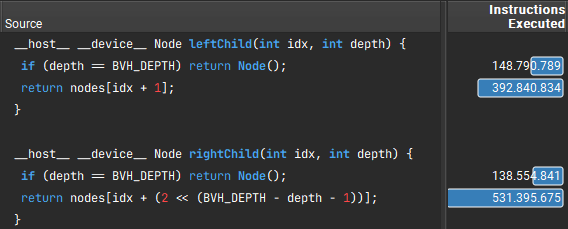
\includegraphics[width=0.5\textwidth]{instructionsexecutedbvh}
	\caption{Nº instrucciones ejecutadas funciones leftChild, rightChild}
	\label{fig:label}
\end{figure}

\begin{figure}[H]
    \centering
	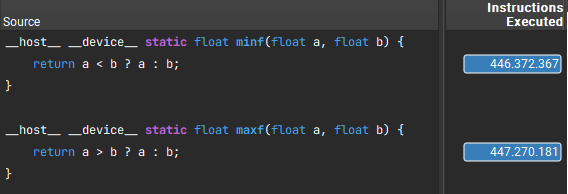
\includegraphics[width=0.5\textwidth]{instructionsexecutedminmax}
	\caption{Nº instrucciones ejecutadas funciones minf/maxf}
	\label{fig:label}
\end{figure}

Estos resultados muestran que la mayoría de las instrucciones ejecutadas se encuentran en el recorrido de los árboles BVH. No es de extrañar que la mayoría de los esfuerzos de optimización del trazado de rayos en el estado del arte residan en estructuras de aceleración más óptimas y compactas. 

NVIDIA Nsight Compute también ofrece advertencias de que partes pueden resultar problemáticas o subóptimas en una arquitectura de GPU en el panel \code{Details}. La ejecución de Eleven Renderer provoca el aviso de un error común en arquitecturas paralelas y es el acceso no secuencial de la memoria. Este fenómeno ocurre cuando los hilos de un wrap no acceden a posiciones contiguas, y en el caso de esta evaluación la advertencia redirige a la parte del código que accede a los hijos del árbol BVH. Esto es de esperar puesto que las estructuras de los árboles no ofrecen buena secuencialidad.

\begin{figure}[H]
    \centering
	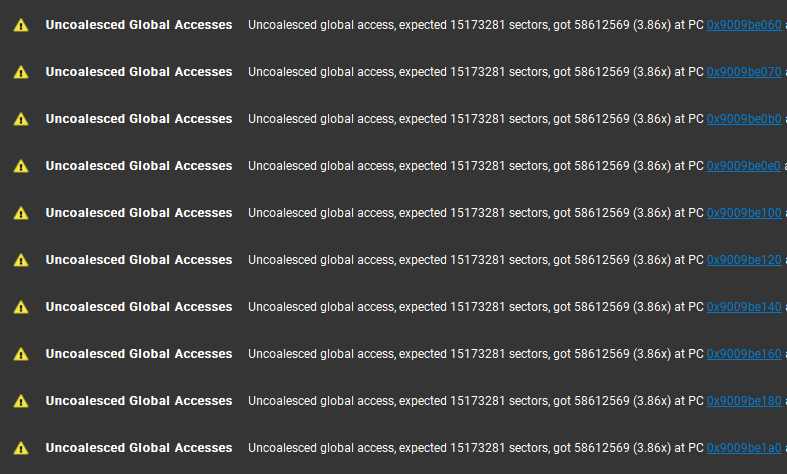
\includegraphics[width=0.7\textwidth]{memoryaccess}
	\caption{Advertencias de acceso no secuencial}
	\label{fig:label}
\end{figure}


\subsection{Análisis Roofline}
	
El modelo Roofline es utilizado en el análisis de eficiencia de aplicaciones de altas prestaciones. Es un modelo que simplifica la visión del hardware y software mostrando un posible techo de eficiencia. NVIDIA Nsight Compute ofrece este análisis para poder analizar posibles deficiencias y optimizaciones.

La línea superior es una cota superior de 29.23 TFLOPS

El análisis de ejecución de Eleven Renderer para precisión simple \autoref{fig:roofline} ha resultado en 0.36 FLOP/byte de intensidad aritmética y 124.47 GFLOPS de eficiencia, mientras que el techo para una intensidad aritmética de 0.36 FLOP/byte está en 330.65 GFLOPS. Esto indica que el algoritmo está corriendo a un 37.6\% de su capacidad máxima teórica según este modelo siempre y cuando la intensidad aritmética no varíe. Este resultado es razonable, indica que no se está infrautilizando el acelerador gráfico, además indica que el algoritmo tiene una gran dependencia de memoria al encontrarse el punto ubicado a la izquierda.

Si se quisiera optimizar más aún este motor, un buen camino sería romper esta dependencia.

\begin{figure}[H]
    \centering
	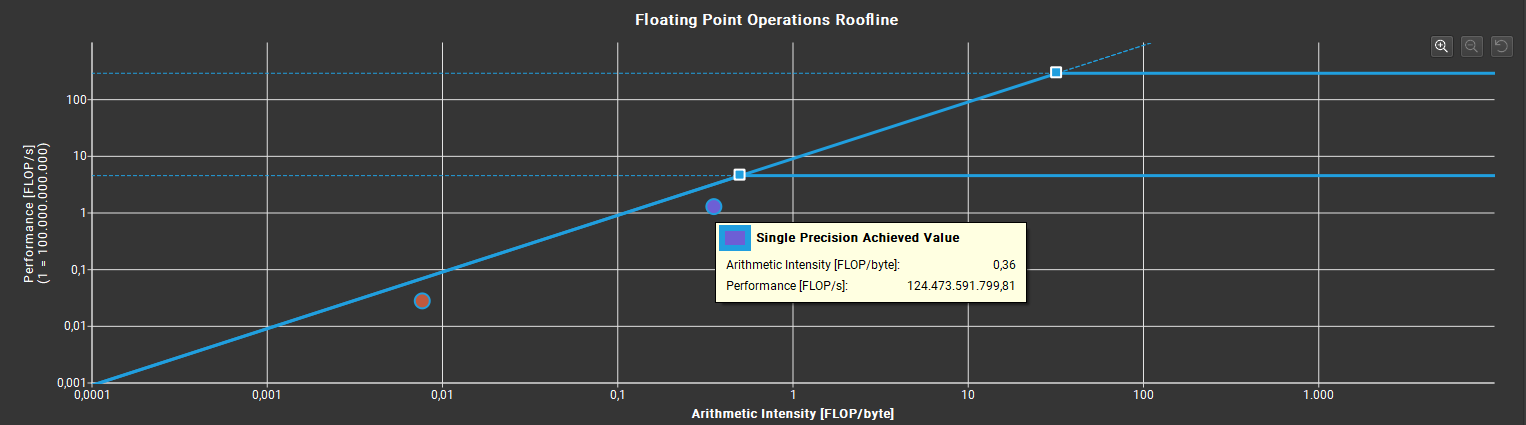
\includegraphics[width=0.9\textwidth]{roofline}
	\caption{Análisis Roofline}
	\label{fig:roofline}
\end{figure}



\chapter{Conclusiones}
	
Desarrollar software con el fin de ser ejecutado en aceleradores gráficos puede ser una tarea relativamente sencilla en una primera instancia. El verdadero interés está conseguir el mayor rendimiento y exprimir estas arquitecturas, teniendo en cuenta sus limitaciones y sus puntos fuertes. 

Haciendo referencia al desarrollo de un motor de renderizado fotorrealista, han habido grandes desafíos. En primer lugar, el renderizado gráfico cuenta con un gran transfondo teórico y matemático del que conviene conocer para poder explotar a fondo cualquier optimización. Este trabajo ha expuesto solo la implementación y la evaluación de este software, sin hacer demasiado hincapié en las bases teóricas. Como se mencionaba en la introducción, Physically based rendering: From theory to implementation \cite{pharr2016physically} es un excelente recurso para esto, denominado por la comunidad como "La biblia del renderizado PBR".

Por otro lado, la programación de Eleven Renderer sido mucho más tediosa de lo esperado. Mientras que mejoras como la construcción de estructuras de aceleración a primera vista podrían imponer por su complejidad, han resultado ser más sencillas de implementar que mejoras más sutiles y simples. Esto es debido a la falta de opciones de depuración en GPU. Mientras que el desarrollo en CPU cuenta con una infinidad de herramientas para analizar el funcionamiento y la ejecución, CUDA solo ofrece un conjunto muy básico de herramientas de análisis y depuración. Así pues, muchas de las soluciones a problemas que han ido surgiendo han tenido que ser resueltas por prueba y error, un enfoque bastante poco óptimo.

Además el enfoque a lo largo del trabajo de implementar todas las opciones posibles en el tiempo dado tiene la desventaja de no contar con una implementación asentada y limpia, si no una en constante cambio y consecuentemente más complicada de analizar. Aún así este enfoque ha hecho posible abarcar todas las bases de un motor de producción mínimo, y aunque en ciertas secciones carece de trasfondo teórico, da una visión global de todos los componentes necesarios.

Algo que se ha observado tras el desarrollo de Eleven Renderer es la carencia en la industria de estándares definidos. Por un lado, no existe una definición de materiales PBR común. El formato .obj es capaz de incluir archivos .mtl, pero éstos sólo contienen información de modelos de sombreado anticuados. Existen propuestas de extender estos formatos pero en la práctica cada programa utiliza su propio formato de archivo.


\section{Trabajo Futuro}
	
Eleven Renderer cuenta con las características visuales mínimas de un motor de producción, así pues deja la puerta abierta a un futuro desarrollo comercial o con fines educativos. No obstante, el siguiente desafío si se quiere seguir produciendo es adaptar la implementación a las suites de software 3d a través de plugins que enlacen las escenas con el motor. 

Queda también una larga lista de mejoras, entre ellas:

\begin{itemize}
	
	\item Mayor variedad de shaders (además del shader de Disney).
	\item Incluir refracción, puesto que por el momento los materiales transparentes son incompatibles con el motor.
	\item Implementar eliminadores de ruido como Open Image Denoise o NVIDIA OptiX™ AI-Accelerated Denoiser.
	\item Añadir un motor de postprocesado más potente con filtros como Bloom o correcciones de color
	\item Añadir más formatos de luces
	\item Experimentar con Embree en CUDA
	
\end{itemize}

Queda pendiente también realizar a fondo un análisis exhaustivo de eficiencia. En el trabajo se han dado pinceladas en este aspecto, por ejemplo la comparación entre búsquedas recursivas o iterativas en GPU, pero hay un centenar de posibles optimizaciones y de prácticas recomendadas para exprimir la eficiencia de la programación en paralelo.

\chapter*{Future work}


\section{Trabajo Futuro}
	

\chapter{Anexo}
	
\section{Manual}
	
Tras compilar el repositorio o haber descargado un ejecutable, es preciso incluir en la línea de comandos tres parámetros. El primero es el directorio donde se encuentra la escena, el segundo es el número de muestras deseado y el tercero el archivo de salida en formato .bmp de la imagen resultante.
	
\subsection{Formato de escenas}
\label{sceneformat}

Debido a la falta de consenso en cuanto a formatos en la industria, se ha utilizado un formato de escenas intentando respetar los estándares más comunes. Así pues una escena se define como un directorio.

Dentro este directorio debe incluir en su interior 3 carpetas

\begin{itemize}
	\item Objects: utilizada para las geometrías en formato .obj. Es necesario que estas geometrías hayan sido trianguladas previamente puesto que el parser desarrollado está limitado a triángulos.
	
	\item Textures: utilizada para las texturas. Actualmente solo se permiten texturas para los atributos: Albedo, Emission, Roughness, Metallic, Normal. Las texturas tienen que estar en formato bmp de 24 bits. El formato de nombre es el siguiente: nombredelmaterial\_tipodemapa.bmp. Por ejemplo: material1\_albedo.bmp, material1\_metallic.bmp. No es necesario que se definan todas las texturas, si no existe alguna se ignorará y se utilizará el valor de color definido en el archivo scene.json. En caso de no existir tampoco ese valor, se utilizará el valor por defecto. Las texturas de albedo y emisión deberán encontrarse en espacio de color sRGB mientras que el resto de texturas deben estar en un espacio lineal. Esto no es respetado por muchos motores de renderizado y es dependiente de la implementación.
	
	\item HDRI: utilizada para los mapas de entorno. Dentro albergará los archivos en formato .hdr de los mapas de entorno.
\end{itemize}

Además será obligatorio incluir un archivo llamado scene.json. Este archivo ha de incluir la información de la escena necesaria. Se muestra un ejemplo como plantilla:

\begin{minipage}[c]{0.95\textwidth}
\begin{lstlisting}
	
{	
'camera' : {'xRes' : 1280, 'yRes' : 720, 'position' : {x : 0, y : 1, z : 2}, 'focalLength' : 0.05, 'focusDistance' : 1, 'aperture' : 2.8},
'materials' : [{'name' : 'mat1'}, {'name' : 'mat2', 'albedo' : {'r' : 1, 'g' : 0, 'b' : 0}, 'roughness' : 0.2}],
'objects' : [{'name' : 'obj1', 'material' : 'mat1'}, {'name' : 'obj2', 'material' : 'mat2'}],
'hdri' : {'name' : 'hdri', 'xOffset' : 0.5},
'pointLights' : [{'position' : {'x' : 0, 'y': 0, 'z': 0}, 'radiance' {'r' : 1, 'g' : 0, 'b' : 0}}]
}
	
\end{lstlisting}
\end{minipage}

El ejemplo mostrado deberá contener dos objetos dentro de la carpeta Objects: obj1.obj y obj2.obj. El material mat1 utilizará las texturas que empiecen por mat1\_...bmp mientras que el mat2 utilizará los valores rgb(1,0,0) para albedo y el valor 0.2 para roughness. Finalmente, se añade una luz puntual en la posición (0,0,0).

Para más ejemplos consultar la carpeta \emph{scenes} del repositorio.

\subsection{Ejemplo de renderizado de escena \emph{ClockCC0}}

Con el fin de demostrar el funcionamiento con un ejemplo real, se ha preparado una escena para la cual, todos los recursos tienen licencia CC0. Esta escena se encuentra en el repositorio y puede ser recreada si se siguen los pasos mostrados en este punto.

Los modelos y texturas utilizados para esta escena son los siguientes:

\begin{itemize}
	\item Modelo de planta: \url{https://polyhaven.com/a/potted_plant_04}
	\item Modelo de mesa: \url{https://polyhaven.com/a/vintage_wooden_drawer_01}
	\item Modelo de reloj: \url{https://polyhaven.com/a/alarm_clock_01}
	\item HDRI de interior: \url{https://polyhaven.com/a/photo_studio_london_hall}
\end{itemize}

Para la ejecución del programa, en el entorno utilizado, ha sido necesario utilizar los siguientes argumentos:
	\code{eleven.exe ''C:$\backslash\backslash$Users$\backslash\backslash$Kike$\backslash\backslash$Desktop$\backslash\backslash$Uni$\backslash\backslash$TFG$\backslash\backslash$Scenes$\backslash\backslash$ClockCC0'' output.bmp 5000}

Tras comenzar el renderizado aparecen dos ventanas, la primera es la consola de salida que se muestra en la \autoref{fig:debugwindow}. Esta ventana contiene datos relevantes en cuanto a la ejecución, como: El progreso de la construcción del BVH, cantidad de memoria utilizada por las geometrías/texturas, eficiencia en kPaths/s, cuanta memoria consume la escena en la GPU y cuanta hay libre, cuántas muestras se han tomado y el tiempo total de ejecución.

Por otro lado, está la ventana de previsualización \autoref{fig:samplewindow}. Esta ventana muestra el progreso visual del render y en la esquina superior izquierda, el número de muestras tomadas por cada píxel hasta el momento.

Finalmente la imagen será guardada como "render.bmp" tras ejecutar las 5000 muestras. En este caso la salida es la \autoref{fig:finalimagewindow}. Este resultado se ha obtenido tras 20 minutos y 39 segundos en una NVIDIA RTX 3090. Con un número mucho menor de muestras es posible seguir obteniendo buenos resultados.

\begin{figure}[H]
    \centering
	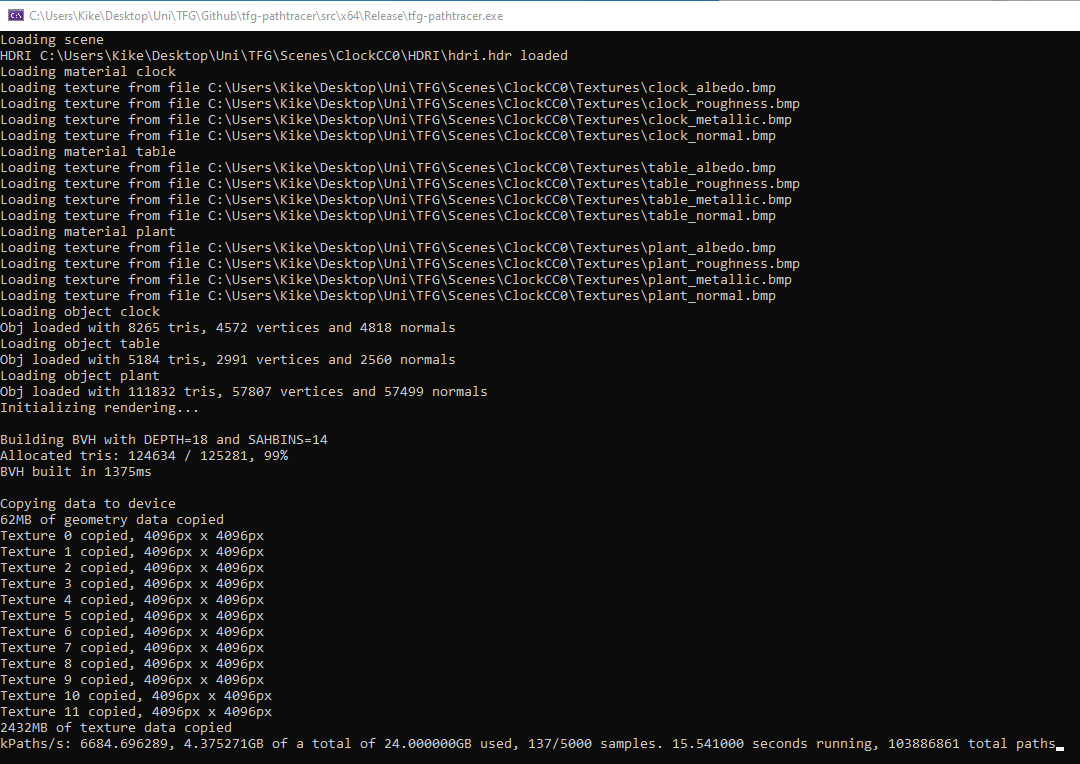
\includegraphics[width=0.9\textwidth]{execdebug}
	\caption{Ventana de depuración}
	\label{fig:debugwindow}
\end{figure}

\begin{figure}[H]
    \centering
	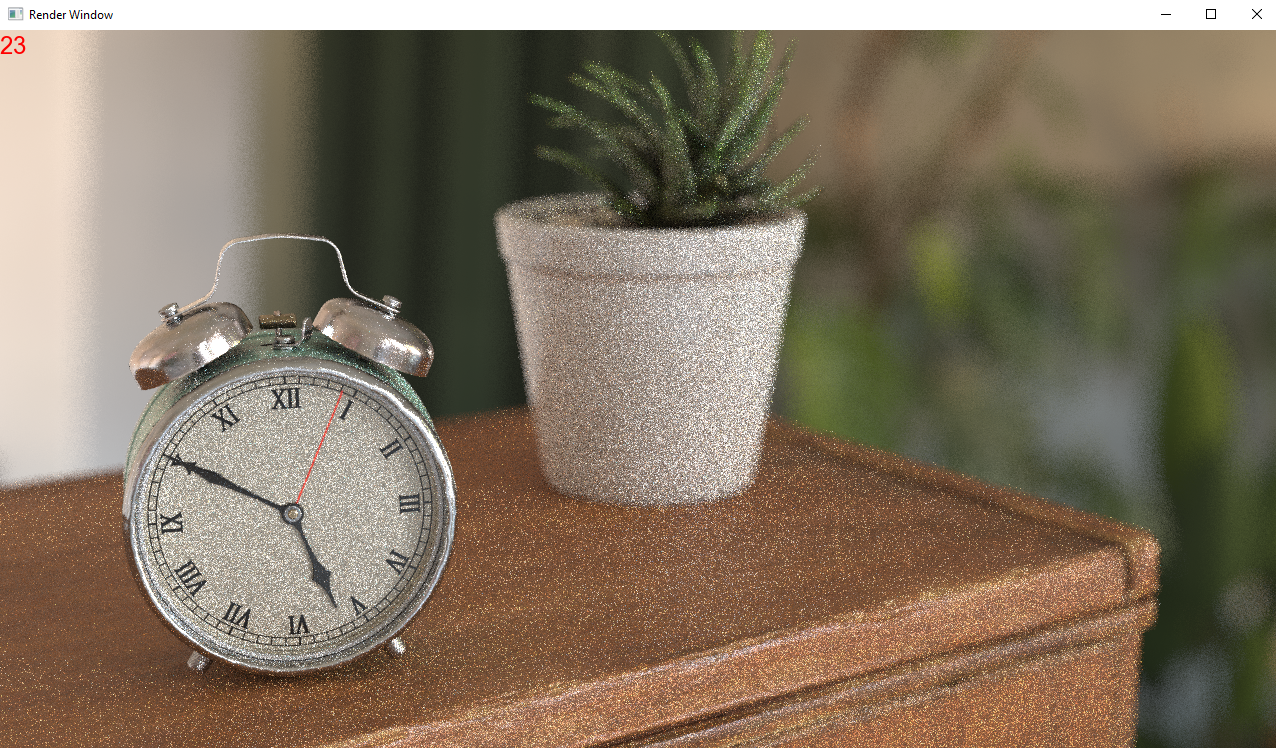
\includegraphics[width=0.9\textwidth]{execsamples}
	\caption{Ventana de previsualización}
	\label{fig:samplewindow}
\end{figure}

\begin{figure}[H]
    \centering
	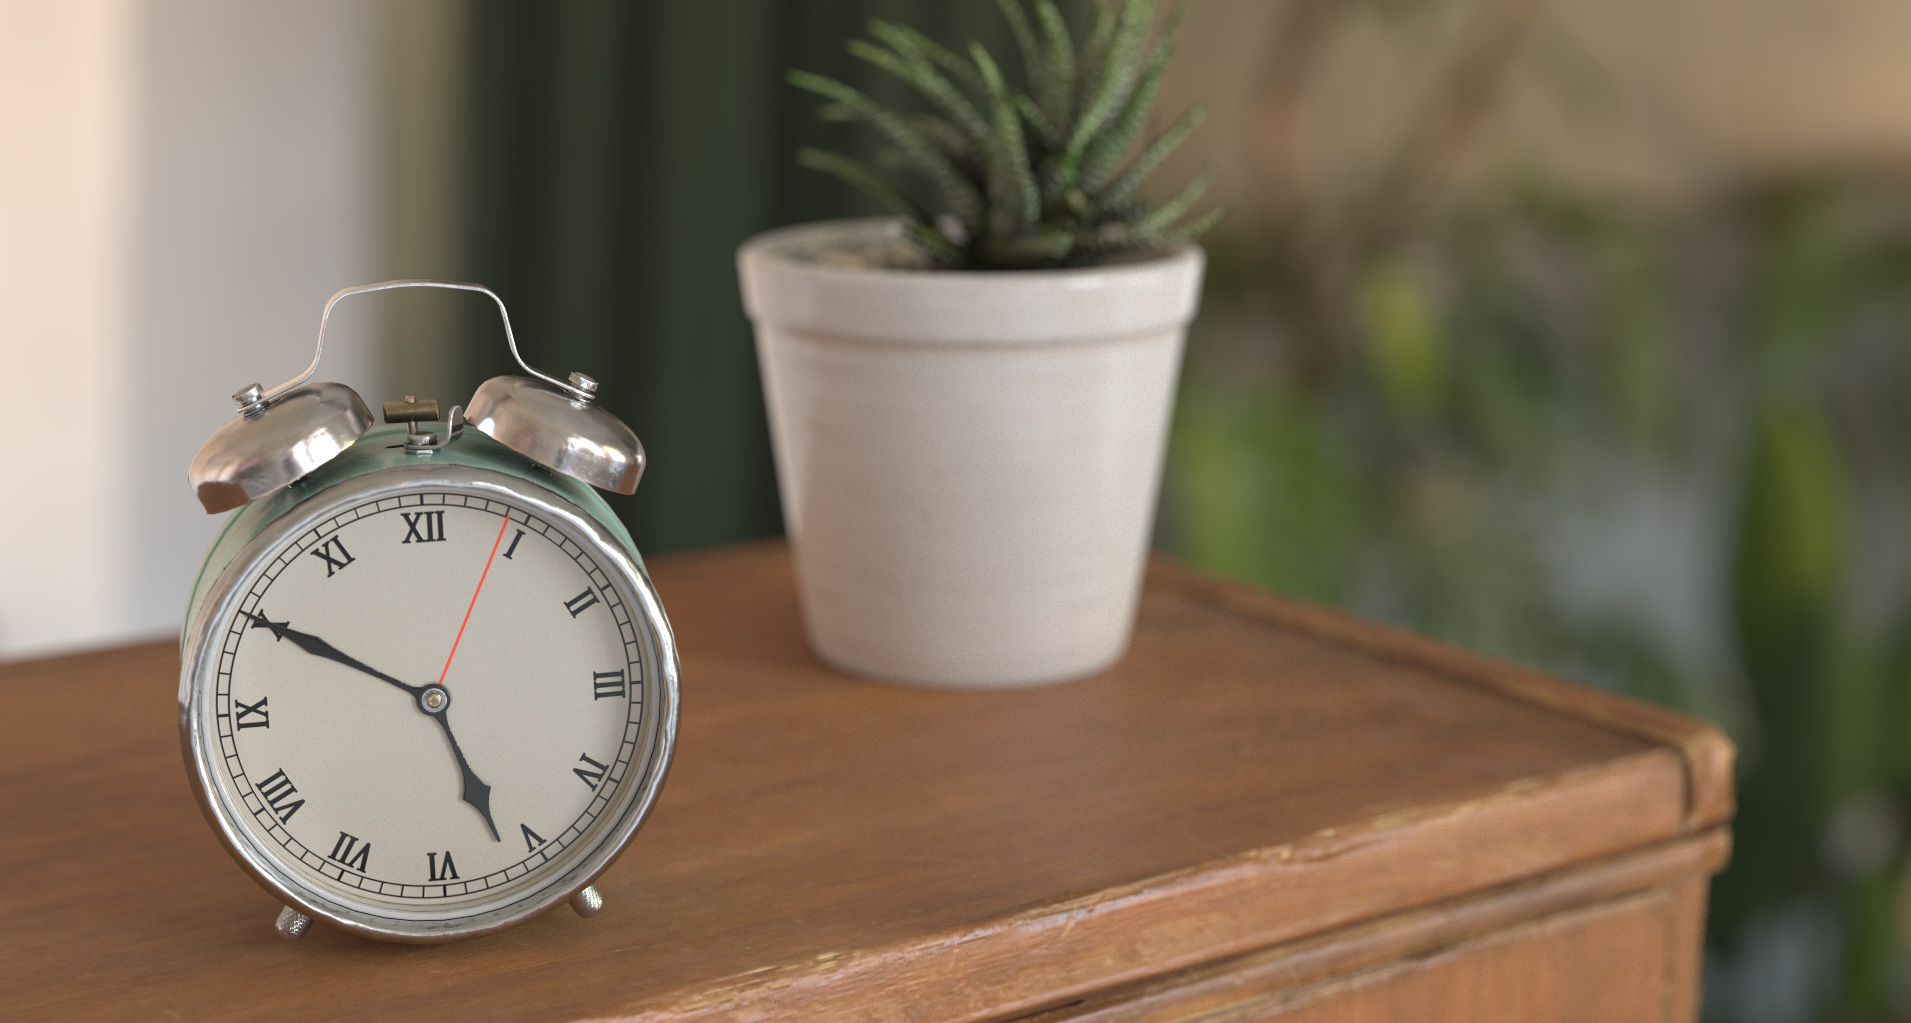
\includegraphics[width=0.9\textwidth]{execfinalimage}
	\caption{Imagen final}
	\label{fig:finalimagewindow}
\end{figure}
	

\bibliographystyle{plain}
\bibliography{refs}
	

 
\end{document}